% ===========================================================================
% MODELO DE RELATORIO  ·  ENE0046 Laboratorio de Eletronica  ·  2026/2
%
% Como usar
%   1. Preencha o bloco IDENTIFICACAO logo abaixo.
%   2. Deixe comentados os autores que nao existirem. Um autor fica centralizado,
%      dois dividem a linha, tres ocupam tercos.
%   3. Substitua o texto de cada secao pelo seu. As orientacoes que estao la
%      dizem o que se espera em cada uma.
%   4. Compile com pdflatex duas vezes, ou com latexmk -pdf.
%
% Estrutura
%   Roteiro 1 nao tem bancada: use so a subsecao 4.1 e a 5.1, e compare o calculo
%   analitico com a simulacao de projeto.
%   Roteiros 2 a 7 usam a estrutura inteira.
%
% O arquivo estilo-relatorio.tex e a imagem logo-unb.png devem estar na mesma
% pasta deste arquivo.
% ===========================================================================
\documentclass[11pt,a4paper]{article}
% !TeX root = modelo-relatorio.tex
% Formatacao do relatorio. Compile o modelo-relatorio.tex, nao este arquivo.
\usepackage[T1]{fontenc}
\usepackage[utf8]{inputenc}
\usepackage{babel}
\usepackage[a4paper,top=1.6cm,bottom=1.8cm,left=2.1cm,right=2.1cm]{geometry}
\usepackage[default]{lato}
\usepackage{amsmath,amssymb}
\usepackage{siunitx}
\usepackage{graphicx}
\usepackage{booktabs,array,longtable,colortbl}
\usepackage{enumitem}
\usepackage{tcolorbox}
\usepackage{xcolor}
\usepackage{tikz}
\usepackage{titlesec}
\usepackage{fancyhdr}
\usepackage{caption}
\usepackage{etoolbox}
\usepackage{placeins}
\usepackage{float}
\usepackage[colorlinks=true,linkcolor=azul,urlcolor=azul,citecolor=azul]{hyperref}
\tcbuselibrary{skins,breakable}

\definecolor{azul}{HTML}{0A4B8C}
\definecolor{azulclaro}{HTML}{E8F0F8}
\definecolor{verde}{HTML}{0B7A4B}
\definecolor{cinza}{HTML}{5B6672}
\definecolor{cinzaclaro}{HTML}{F4F6F8}
\definecolor{vinho}{HTML}{B04A4A}
\definecolor{vinhoclaro}{HTML}{FBF2F2}

\sisetup{output-decimal-marker={,}, per-mode=symbol}
\setlength{\parindent}{0pt}
\setlength{\parskip}{6pt plus 1pt}
\setlist{itemsep=3pt, topsep=4pt, parsep=0pt, leftmargin=1.3em}
\renewcommand{\arraystretch}{1.25}
\linespread{1.06}

% ---- secoes numeradas com marcador colorido -------------------------------
\titleformat{\section}[hang]
  {\Large\bfseries\color{azul}}
  {\raisebox{-1pt}{\tikz\node[fill=azul,text=white,rounded corners=2pt,
     inner sep=3pt,minimum width=20pt,align=center]{\bfseries\thesection};}}
  {10pt}{}
\titlespacing*{\section}{0pt}{16pt plus 3pt}{6pt}
\titleformat{\subsection}{\large\bfseries\color{cinza}}{\thesubsection}{8pt}{}
\titlespacing*{\subsection}{0pt}{11pt plus 2pt}{3pt}

% ---- legendas -------------------------------------------------------------
\captionsetup{font=small,labelfont={bf,color=azul},labelsep=period,skip=6pt}

% ---- identificacao --------------------------------------------------------
\newcommand{\autorA}{}\newcommand{\matA}{}
\newcommand{\autorB}{}\newcommand{\matB}{}
\newcommand{\autorC}{}\newcommand{\matC}{}
\newcommand{\autorum}[2]{\renewcommand{\autorA}{#1}\renewcommand{\matA}{#2}}
\newcommand{\autordois}[2]{\renewcommand{\autorB}{#1}\renewcommand{\matB}{#2}}
\newcommand{\autortres}[2]{\renewcommand{\autorC}{#1}\renewcommand{\matC}{#2}}

\newcommand{\disciplina}{CIC0236 · Teleinformática e Redes 2}
\newcommand{\semestre}{2026/2}
\newcommand{\turma}{}
\newcommand{\gruponum}{}
\newcommand{\roteironum}{}
\newcommand{\roteirotema}{}
\newcommand{\aturma}[1]{\renewcommand{\turma}{#1}}
\newcommand{\grupo}[1]{\renewcommand{\gruponum}{#1}}
\newcommand{\roteiro}[2]{\renewcommand{\roteironum}{#1}\renewcommand{\roteirotema}{#2}}

\newcommand{\umautor}[2]{%
  \begin{minipage}[t]{\dimexpr\linewidth-4pt\relax}\centering
    \parbox[t][30pt][t]{\linewidth}{\centering
      {\fontsize{10.5}{12.5}\selectfont #1}}\\[-2pt]
    {\color{cinza}\fontsize{9}{11}\selectfont\texttt{#2}}
  \end{minipage}}

\newcounter{nautores}
\newcommand{\blocoautores}{%
  \setcounter{nautores}{0}%
  \ifdefempty{\autorA}{}{\stepcounter{nautores}}%
  \ifdefempty{\autorB}{}{\stepcounter{nautores}}%
  \ifdefempty{\autorC}{}{\stepcounter{nautores}}%
  \ifnum\value{nautores}=0
    \begin{center}\color{vinho}\bfseries
      Preencha ao menos um autor no preâmbulo do arquivo.
    \end{center}
  \else
    \begin{center}
    \ifcase\value{nautores}\or
      % --- um autor: ocupa o centro
      \begin{minipage}{0.5\textwidth}\umautor{\autorA}{\matA}\end{minipage}%
    \or
      % --- dois autores: metades
      \begin{minipage}{0.42\textwidth}\umautor{\autorA}{\matA}\end{minipage}\hspace{0.04\textwidth}%
      \begin{minipage}{0.42\textwidth}\umautor{\autorB}{\matB}\end{minipage}%
    \or
      % --- tres autores: tercos
      \begin{minipage}{0.31\textwidth}\umautor{\autorA}{\matA}\end{minipage}\hspace{0.015\textwidth}%
      \begin{minipage}{0.31\textwidth}\umautor{\autorB}{\matB}\end{minipage}\hspace{0.015\textwidth}%
      \begin{minipage}{0.31\textwidth}\umautor{\autorC}{\matC}\end{minipage}%
    \fi
    \end{center}
  \fi}

% ---- cabecalho do relatorio -----------------------------------------------
\newcommand{\capa}{%
\begin{tcolorbox}[colback=azul,colframe=azul,boxrule=0pt,arc=4pt,
  left=16pt,right=16pt,top=13pt,bottom=13pt]
\color{white}
\begin{minipage}{0.76\textwidth}
  {\fontsize{9}{11}\selectfont\textbf{\MakeUppercase{\disciplina{} · \semestre{}}}}\\[6pt]
  {\fontsize{22}{25}\selectfont\bfseries Relatório da Entrega \roteironum}\\[3pt]
  {\fontsize{12.5}{15}\selectfont \roteirotema}
\end{minipage}\hfill
\begin{minipage}{0.2\textwidth}\raggedleft
  \colorbox{white}{\hspace{2pt}\raisebox{-2pt}{
\includegraphics[height=30pt]{logo-unb.png}}\hspace{2pt}}
\end{minipage}
\end{tcolorbox}
\vspace{10pt}
\blocoautores
\ifdefempty{\turma}{}{%
  \begin{center}{\color{cinza}\fontsize{9}{11}\selectfont Turma \turma}\end{center}}
\ifdefempty{\gruponum}{}{%
  \begin{center}{\color{cinza}\fontsize{9}{11}\selectfont Grupo \gruponum}\end{center}}
\vspace{4pt}
{\color{azulclaro}\hrule height 2pt}
\vspace{2pt}}

% ---- caixas auxiliares ----------------------------------------------------
\newtcolorbox{formula}{colback=azulclaro,colframe=azul,boxrule=0.8pt,arc=3pt,
  left=12pt,right=12pt,top=9pt,bottom=9pt}
\newtcolorbox{nota}[1]{colback=cinzaclaro,colframe=cinza,boxrule=0.8pt,arc=3pt,
  left=10pt,right=10pt,top=7pt,bottom=7pt,
  title={\textbf{#1}},fonttitle=\small\bfseries,coltitle=white,colbacktitle=cinza}
\newenvironment{resumo}
  {\vspace{6pt}\begin{center}\begin{minipage}{0.92\textwidth}
   \begin{tcolorbox}[colback=cinzaclaro,colframe=cinzaclaro,boxrule=0pt,arc=3pt,
     left=14pt,right=14pt,top=10pt,bottom=10pt,
     borderline west={2.5pt}{0pt}{azul}]
   {\color{azul}\fontsize{8}{10}\selectfont\textbf{RESUMO}}\\[4pt]
   \small}
  {\end{tcolorbox}\end{minipage}\end{center}\vspace{2pt}}

\newtcolorbox{espec}{colback=azulclaro,colframe=azul,boxrule=0.8pt,arc=3pt,
  left=12pt,right=12pt,top=9pt,bottom=9pt,
  title={\textbf{Especificação da matrícula}},fonttitle=\bfseries,
  coltitle=white,colbacktitle=azul}

% ---- rodape ---------------------------------------------------------------
\pagestyle{fancy}\fancyhf{}
\renewcommand{\headrulewidth}{0pt}
\renewcommand{\footrulewidth}{0.4pt}
\fancyfoot[L]{\color{cinza}\fontsize{8}{10}\selectfont \disciplina{} · \semestre{} · Entrega \roteironum}
\fancyfoot[R]{\color{cinza}\fontsize{8}{10}\selectfont \thepage}

\newlist{referencias}{itemize}{1}
\setlist[referencias]{label={}, leftmargin=1.1em, itemindent=-1.1em,
                     itemsep=3pt, topsep=2pt, parsep=0pt}

\newcommand{\mat}[1]{\texttt{\textbf{#1}}}


% --------------------------- IDENTIFICACAO ---------------------------------
\roteiro{3}{RTT Adaptativo}
\aturma{01}
\grupo{12}

\autorum{Enzo Morrone de Azevedo Muniz}{221035442}
\autordois{Luca Valderramos Cirino}{211066140}
\autortres{Raul Myron Silva Amorim}{200049712}
% ---------------------------------------------------------------------------

\newcommand{\pend}[1]{\textcolor{red}{#1}}
\begin{document}
\capa

\begin{resumo}
Este relatório conclui o projeto RDT-UnB (\textit{Reliable Data Transfer over
UDP}) apresentando a etapa de RTT adaptativo: o timeout deixa de ser fixo em
\SI{500}{\milli\second} e passa a ser calculado por segmento com a fórmula do
TCP ($RTT_{est} + 4 \cdot DevRTT$, estimada por EWMA com $\alpha = 0.125$ e
$\beta = 0.25$), incluindo o Karn's algorithm, piso de RTO configurável
(\SI{100}{\milli\second}) e backoff da RFC 6298 (dobra apenas o RTO, limitado a
\SI{1}{\second}). Com a mesma sequência de perdas (mesma seed), o SR com janela
16 e timeout adaptativo atingiu \SI{1788.77}{\kilo\bit\per\second} contra
\SI{1139.13}{\kilo\bit\per\second} do fixo a \SI{5}{\percent} de perda
(\SI{57}{\percent} de ganho) e \SI{1525.33}{\kilo\bit\per\second} contra
\SI{704.72}{\kilo\bit\per\second} a \SI{10}{\percent} (\SI{116}{\percent}); sem
perdas, os dois modos empatam. No comparativo geral, o SR-16 adaptativo foi o
melhor protocolo do projeto (\SI{2089.87}{\kilo\bit\per\second} no arquivo
\textit{large}). Todo o código está no
repositório \url{https://github.com/luca2453/rdt-unb}.
\end{resumo}

% RELATÓRIO FINAL: 
%
% Relatório final em PDF (máximo 15 páginas), contendo a evolução completa do projeto,  
% das três entregas, com análise comparativa entre todas as implementações.
%
% Estrutura obrigatória do relatório:


\section{Introdução}

%%%%%%%%%%%%%%%%%%%%%%%%%%%%%%%%%%%%%%%%%%%%%%%%%%%%%%%%%%%%%%%%%%%%%%%%%%%%%%%%
% 1. Introdução e evolução do projeto
% Descreva brevemente a jornada: o que foi implementado em cada entrega, 
% quais dificuldades foram encontradas e como foram resolvidas. Não é um resumo 
% burocrático — é uma narrativa técnica de como o grupo evoluiu de um cliente 
% SAW simples até um cliente com RTT adaptativo.
%%%%%%%%%%%%%%%%%%%%%%%%%%%%%%%%%%%%%%%%%%%%%%%%%%%%%%%%%%%%%%%%%%%%%%%%%%%%%%%%

Este é o relatório 3 de 3 no projeto de criar transferência confiável de dados
no UDP, sendo chamado: \textit{Reliable Data Transfer over UDP – RDT-UnB}.

Na primeira etapa, já foi implementada a transferência confiável por meio do protocolo
SAW (\textit{Stop-and-Wait}). Resumidamente, apenas um pacote está em trânsito em
cada momento e, em caso de timeout, ele é solicitado novamente. O SAW simplifica 
a implementação, mas é muito impactado pelo \textit{Round Trip Time} (RTT) da
transmissão, o que faz ele ter uma largura de banda baixa.

Na segunda etapa, o problema da largura de banda é parcialmente resolvido com a adoção
de janelas de transferência em duas abordagens, a \textit{Go-back-N} (GBN) e
\textit{Selective Repeat} (SR). Ambas se diferem apenas na forma de tratar timeouts.
Sendo N o tamanho da janela, no GBN, em caso de timeout, ele resolicita N pacotes, 
começando pelo pacote que sofreu timeout. Já o SR, apenas solicita o 1 pacote que sofreu
timeout.

As implicações disso são: o GBN tem uma lógica mais simples de implementar, mas tende a
ter um desempenho pior que o SR visto que as perdas de pacotes tendem a ser isoladas,
trazendo pouco benefício ao resolicitar todos os N-1 pacotes seguintes. Além disso,
esses protocolos ainda podem sofrer muito com tempos de timeout inadequados.

Por isso, nesta terceira etapa, é implementado uma adição a estes protocolos,
a de RTT Adaptativo. Ou seja, ao invés do tempo de timeout ser definido previamente,
o protocolo RDT-UnB passa a ajustar o timeout de forma dinâmica, refletindo as condições
atuais da rede. Assim, espera-se que os timeouts tenham menos penalização à taxa de
transmissão, possibilitando um aumento na largura de banda.

Este relatório está dividido em 4 seções principais: na implementação é dito como foi feito o código que implementa o protocolo;
na comparação, tem-se dados com os protocolos com e sem timeout fixo; na análise Wireshark, tem-se dados coletados da ferramenta;
e por último na visão integrada, tem-se dados consolidativos.

\section{RTT Adaptativo - Implementação}

%%%%%%%%%%%%%%%%%%%%%%%%%%%%%%%%%%%%%%%%%%%%%%%%%%%%%%%%%%%%%%%%%%%%%%%%%%%%%%%%
% 2. RTT Adaptativo — implementação
%
% Descreva a fórmula EWMA implementada:
% Justifique os valores de α e β escolhidos:   mostre o impacto nos dados com os valores escolhidos. 
% Gráfico do RTT estimado vs RTT medido por segmento,  mostrando a convergência do estimador ao longo da transferência
% Gráfico do timeout ao longo da transferência, mostrando como ele se adapta a variações de RTT
%%%%%%%%%%%%%%%%%%%%%%%%%%%%%%%%%%%%%%%%%%%%%%%%%%%%%%%%%%%%%%%%%%%%%%%%%%%%%%%%


% •       Medir o RTT de cada segmento (tempo entre REQ e DATA correspondente)
% •       Calcular o RTT estimado usando EWMA: RTT_est = (1 - α) × RTT_est + α × RTT_medido
% •       Calcular o DevRTT (desvio): DevRTT = (1 - β) × DevRTT + β × |RTT_medido - RTT_est|
% •       Definir timeout = RTT_est + 4 × DevRTT (fórmula do TCP)


A implementação do RTT Adaptativo se deu por meio do seguinte processo:

Primeiro, a cada segmento, é medido o RTT . Depois, usando médias móveis é obtido os valores $RTT_{est}$ e $DevRTT$ usando as seguintes fórmulas:

\begin{equation}
RTT_{est} = (1 - \alpha) * RTT_{est} + \alpha * RTT_{medido}
\label{eq:EWMA}
\end{equation}

\begin{equation}
	DevRTT = (1 - \beta) * DevRTT + \beta * | RTT_{medido} - RTT_{est} |
\label{eq:Devrtt}
\end{equation}

Essas fórmulas são simplesmente uma implementação de uma média móvel exponencial com pesos. 
Dessa forma, para estimar o valor ideal do RTT, evita-se mudanças bruscas devido a média, mas também permite 
mudanças um pouco mais rápidas devido a natureza exponencial da média, que possui os termos mais
recentes com mais peso.

Depois, é definido o novo timeout seguindo a relação:

\begin{equation}
	\text{timeout} = RTT_{est} + 4 * DevRTT
	\label{eq:novo_timeout}
\end{equation}

Essa equação \ref{eq:novo_timeout} é a mesma fórmula usada pelo TCP.

Com isso, resta apenas definir valores razoáveis para $\alpha$ e $\beta$. O grupo decidiu ir com $\alpha = 0.125$ e $\beta = 0.25$. Quanto maior estes valores,
mais rápido o protocolo se adapta as mudanças. Esses valores tenderam a ter o melhor desempenho nos testes realizados, visto que as condições de rede
não costumam mudar muito durante os testes.

\label{sec:impl_rtt}
O timeout adaptativo foi aplicado ao GBN e SR e é escolhido na linha de
comando com \texttt{-{}-timeout fixed|adaptive}; os pesos são definidos por
\texttt{-{}-alpha} e \texttt{-{}-beta}. Assim, a mesma versão do cliente gera os
dois cenários comparados na Seção~\ref{sec:fixo_adapt}, e a única diferença entre
eles é a regra do timeout. Dois detalhes da implementação merecem destaque:

\begin{itemize}
	\item \textbf{Valor inicial.} O $RTT_{est}$ inicial é o RTT medido pelo
		\textit{ping} que abre a sessão, e o $DevRTT$ começa com metade desse
		valor. Isso garante um timeout conservador para a primeira janela de
		segmentos, antes de existirem amostras por segmento.
	\item \textbf{Piso e backoff (RFC 6298).} O timeout nunca fica abaixo de um
		piso configurável (\texttt{-{}-min-rto}, padrão de \SI{100}{\milli\second}),
		pois a fórmula sozinha convergia para valores menores que o maior RTT
		observado na sessão. A cada \textit{timeout} real, o RTO dobra —
		apenas o RTO, mantendo o estimador EWMA intacto, como no TCP real —,
		limitado a um teto de \SI{1}{\second}, e volta a ser calculado pela
		fórmula assim que chega uma amostra válida (o Karn's algorithm impede
		que retransmissões alimentem o estimador). Perdas simuladas não geram
		backoff, pois nelas não ocorre timeout: a recuperação fica a cargo do
		timer real do segmento.
\end{itemize}

Todo segmento registra no CSV o RTT medido (\texttt{rtt\_ms}), o RTT estimado
naquele instante (\texttt{rtt\_estimated\_ms}) e o timeout em vigor quando ele foi
pedido (\texttt{timeout\_ms}), o que permite reconstruir a evolução do estimador
segmento a segmento.

\section{Comparação entre timeout fixo e adaptativo}
\label{sec:fixo_adapt}
Para isolar o efeito do timeout, o mesmo protocolo (SR com janela 16) foi
executado no arquivo \textit{large} com timeout fixo de \SI{500}{\milli\second} e
com timeout adaptativo, sob 5\,\% e 10\,\% de perda simulada e com a mesma
\textit{seed}. Assim, os dois casos sofrem exatamente a mesma sequência de
descartes, e as diferenças da Tabela~\ref{tab:fixo_adapt} se devem apenas à regra
de timeout.

\begin{table}[H]
\centering
\caption{SR-16, arquivo \textit{large}: timeout fixo $\times$ adaptativo (mesma seed de perda).}
\label{tab:fixo_adapt}
\small
\begin{tabular}{@{}llrrr@{}}
\toprule
Perda & Timeout & Retransmissões & Tempo total (s) & Throughput médio (kbps) \\
\midrule
5\,\%  & fixo       & 1109 & 73,64  & 1139,13 \\
5\,\%  & adaptativo & 1109 & 46,90  & 1788,77 \\
10\,\% & fixo       & 2360 & 119,03 & 704,72 \\
10\,\% & adaptativo & 2357 & 55,00  & 1525,33 \\
\bottomrule
\end{tabular}
\end{table}

Com a mesma quantidade de perdas (mesma seed), o ganho do adaptativo vem
exclusivamente de quanto tempo se espera a cada perda: com timeout fixo de
\SI{500}{\milli\second}, cada segmento perdido custa meio segundo de janela
parada; no adaptativo, a retransmissão parte do piso de \SI{100}{\milli\second}
(ou pouco acima, com os picos de backoff), cerca de 5 vezes menos. O efeito
cresce com a taxa de perda: a \SI{5}{\percent} o adaptativo foi
\SI{57}{\percent} mais rápido e a \SI{10}{\percent}, \SI{116}{\percent}.

\begin{figure}[H]
\centering
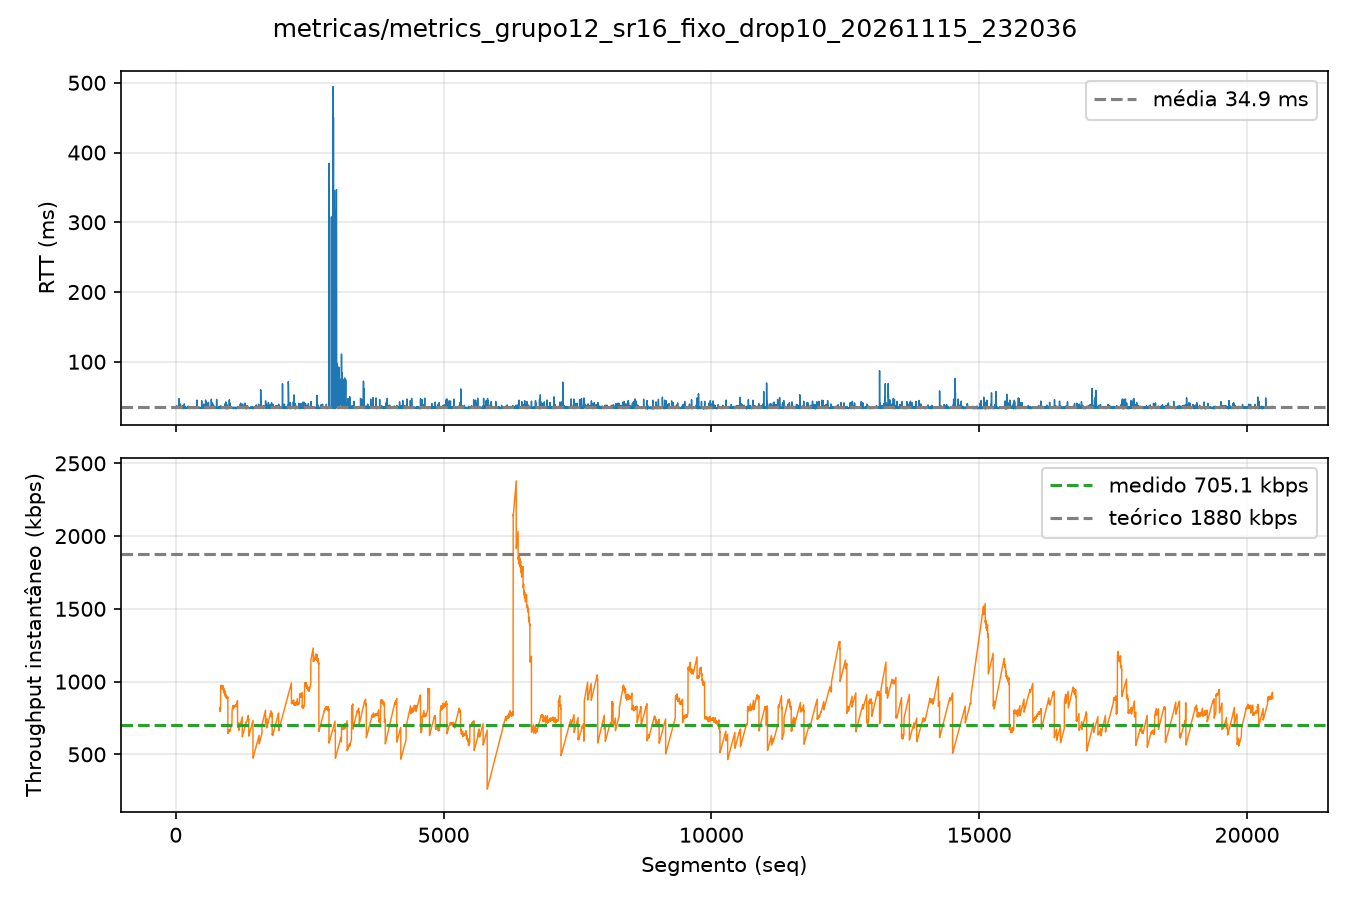
\includegraphics[width=0.85\linewidth]{imagens/sr16_fixo_10.png}
\caption{SR-16, arquivo \textit{large}, 10\,\% de perda, timeout fixo
(\SI{500}{\milli\second}): RTT e \textit{throughput} agregado (média móvel de
3~s). RTT médio de 34,9~ms; 2360 retransmissões em 119~s.}
\label{fig:sr_fixo10}
\end{figure}

\begin{figure}[H]
\centering
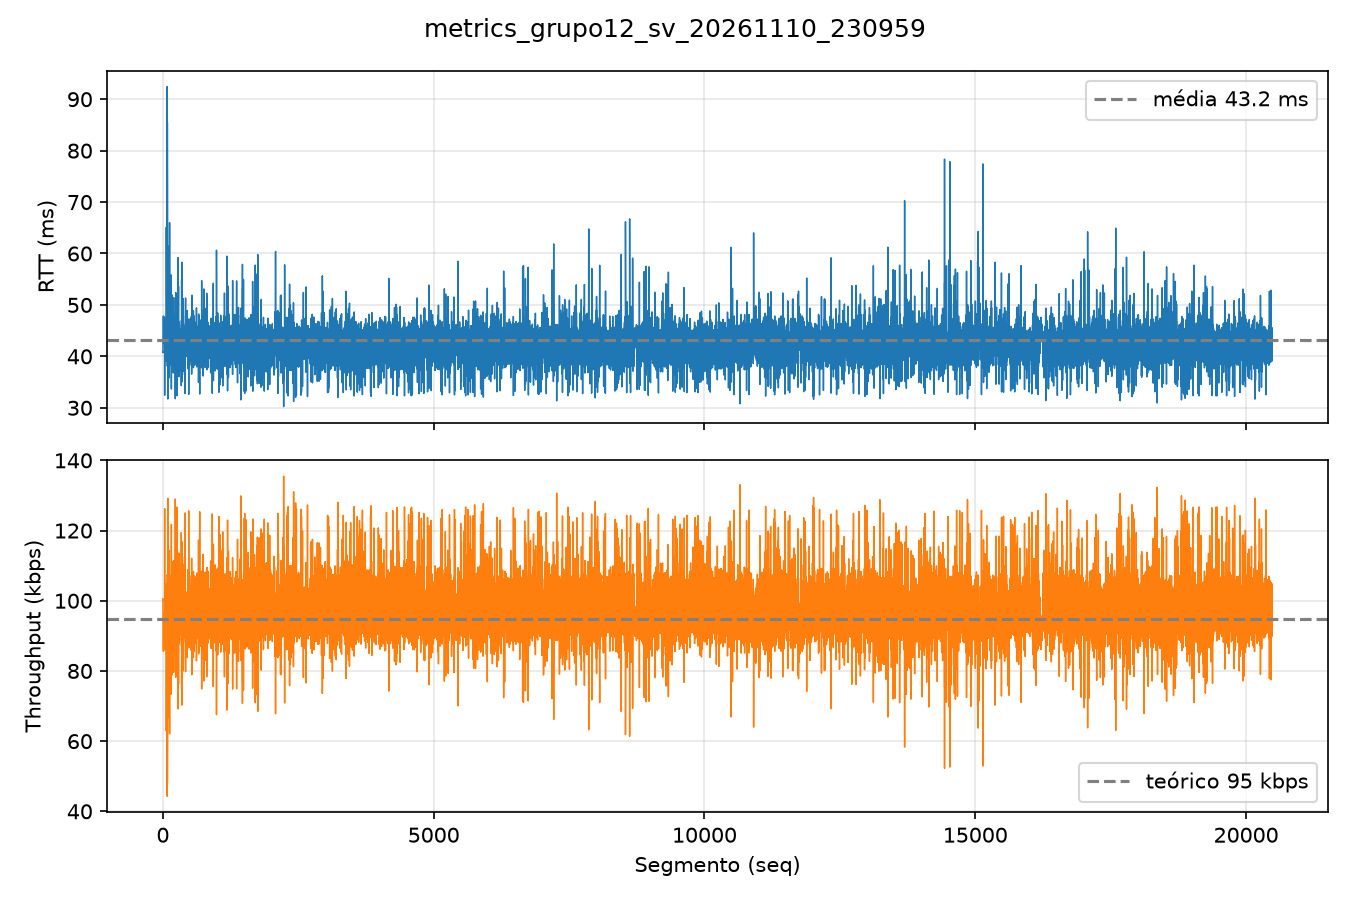
\includegraphics[width=0.85\linewidth]{imagens/sr16_adapt_10.png}
\caption{SR-16, arquivo \textit{large}, 10\,\% de perda, timeout adaptativo:
mesma sequência de perdas da Figura~\ref{fig:sr_fixo10}. O painel de RTT, em
escala log, mostra o RTO no piso de \SI{100}{\milli\second} com os picos de
backoff (200--400~ms) exatamente nos segmentos que estouraram o timer; RTT
médio de 30,6~ms; 2357 retransmissões em 55~s.}
\label{fig:sr_adapt10}
\end{figure}

A Figura~\ref{fig:sr_adapt10} ilustra a vantagem: cada pico vermelho do RTO
marcado no painel de RTT é um timeout, recuperado em ~\SI{100}{\milli\second}
(piso) ou até \SI{400}{\milli\second} (após backoffs consecutivos) — enquanto o
modo fixo da Figura~\ref{fig:sr_fixo10} paga \SI{500}{\milli\second} por cada
um desses eventos. Mesmo com o mesmo número de perdas, o adaptativo mantém a
janela em voo por muito mais tempo.

\paragraph{Quando o adaptativo vale mais a pena?} A vantagem cresce com a taxa
de perda: com a mesma quantidade de retransmissões, cada perda custa ao
adaptativo o RTO corrente (piso de \SI{100}{\milli\second} na prática, com
picos de backoff em rajadas) e ao fixo os \SI{500}{\milli\second} cheios — nos
dados da Tabela~\ref{tab:fixo_adapt}, \SI{57}{\percent} de ganho a
\SI{5}{\percent} de perda e \SI{116}{\percent} a \SI{10}{\percent}. Ele também
é a única opção segura quando o RTT muda durante a transferência (por exemplo,
numa rede móvel), porque um valor fixo menor que o RTT geraria retransmissões
falsas e um valor muito maior desperdiçaria tempo.

\paragraph{Quando o fixo é suficiente?} Sem perda, o timeout nunca chega a
estourar, então o valor não influencia o resultado, desde que seja maior que o
maior RTT da rede. Nesse cenário os dois modos têm desempenho praticamente
igual nas execuções de \textit{small} da Seção~\ref{sec:integrada} (fixo de 2084 vs adaptativo de
1982~kbps), e o fixo tem a vantagem de ser mais simples.


%%%%%%%%%%%%%%%%%%%%%%%%%%%%%%%%%%%%%%%%%%%%%%%%%%%%%%%%%%%%%%%%%%%%%%%%%%%%%%%%
% 3. Comparação entre timeout fixo e adaptativo
%
% Execute o mesmo protocolo (GBN ou SR, à escolha do grupo) com timeout fixo e com timeout adaptativo, sob perda de 5% e 10%
% Tabela comparando: número de retransmissões, tempo total, throughput médio
% Explique: em que situação o timeout adaptativo tem mais vantagem? Em que situação o timeout fixo é suficiente?
%%%%%%%%%%%%%%%%%%%%%%%%%%%%%%%%%%%%%%%%%%%%%%%%%%%%%%%%%%%%%%%%%%%%%%%%%%%%%%%%

\section{Analise Wireshark}

%%%%%%%%%%%%%%%%%%%%%%%%%%%%%%%%%%%%%%%%%%%%%%%%%%%%%%%%%%%%%%%%%%%%%%%%%%%%%%%%
% 4. Análise Wireshark
%
% Capture o tráfego UDP durante uma transferência com o arquivo large
% Filtro: udp and host 137.131.178.229
% Screenshots obrigatórios com anotações:
% Screenshot 1: visão geral da sessão completa (HELLO → sequência de REQs → FIN → DONE)
% Screenshot 2: zoom em pelo menos 2 eventos de retransmissão — mostre o REQ original e o REQ retransmitido com o delta de tempo entre eles
% Screenshot 3: correlação entre um evento do Wireshark (timestamp) e a linha correspondente no CSV
% Meça o RTT diretamente no Wireshark (tempo entre REQ e DATA) e compare com o RTT registrado pelo cliente no CSV — os valores devem ser próximos; se não forem, explique a diferença
%%%%%%%%%%%%%%%%%%%%%%%%%%%%%%%%%%%%%%%%%%%%%%%%%%%%%%%%%%%%%%%%%%%%%%%%%%%%%%%%

Foi registrado no Wireshark, uma transferência usando o RTT Adaptativo usando o
GBN com uma janela de tamanho 16 na transferência do arquivo large. 
É sugerido ao leitor usar a feramenta de zoom de seu leitor de pdf devido a densidade de informação das imagens.
Foi utilizado a função de comentários do wireshark para rotular alguns dos pacotes.

\begin{figure}[H]
\centering
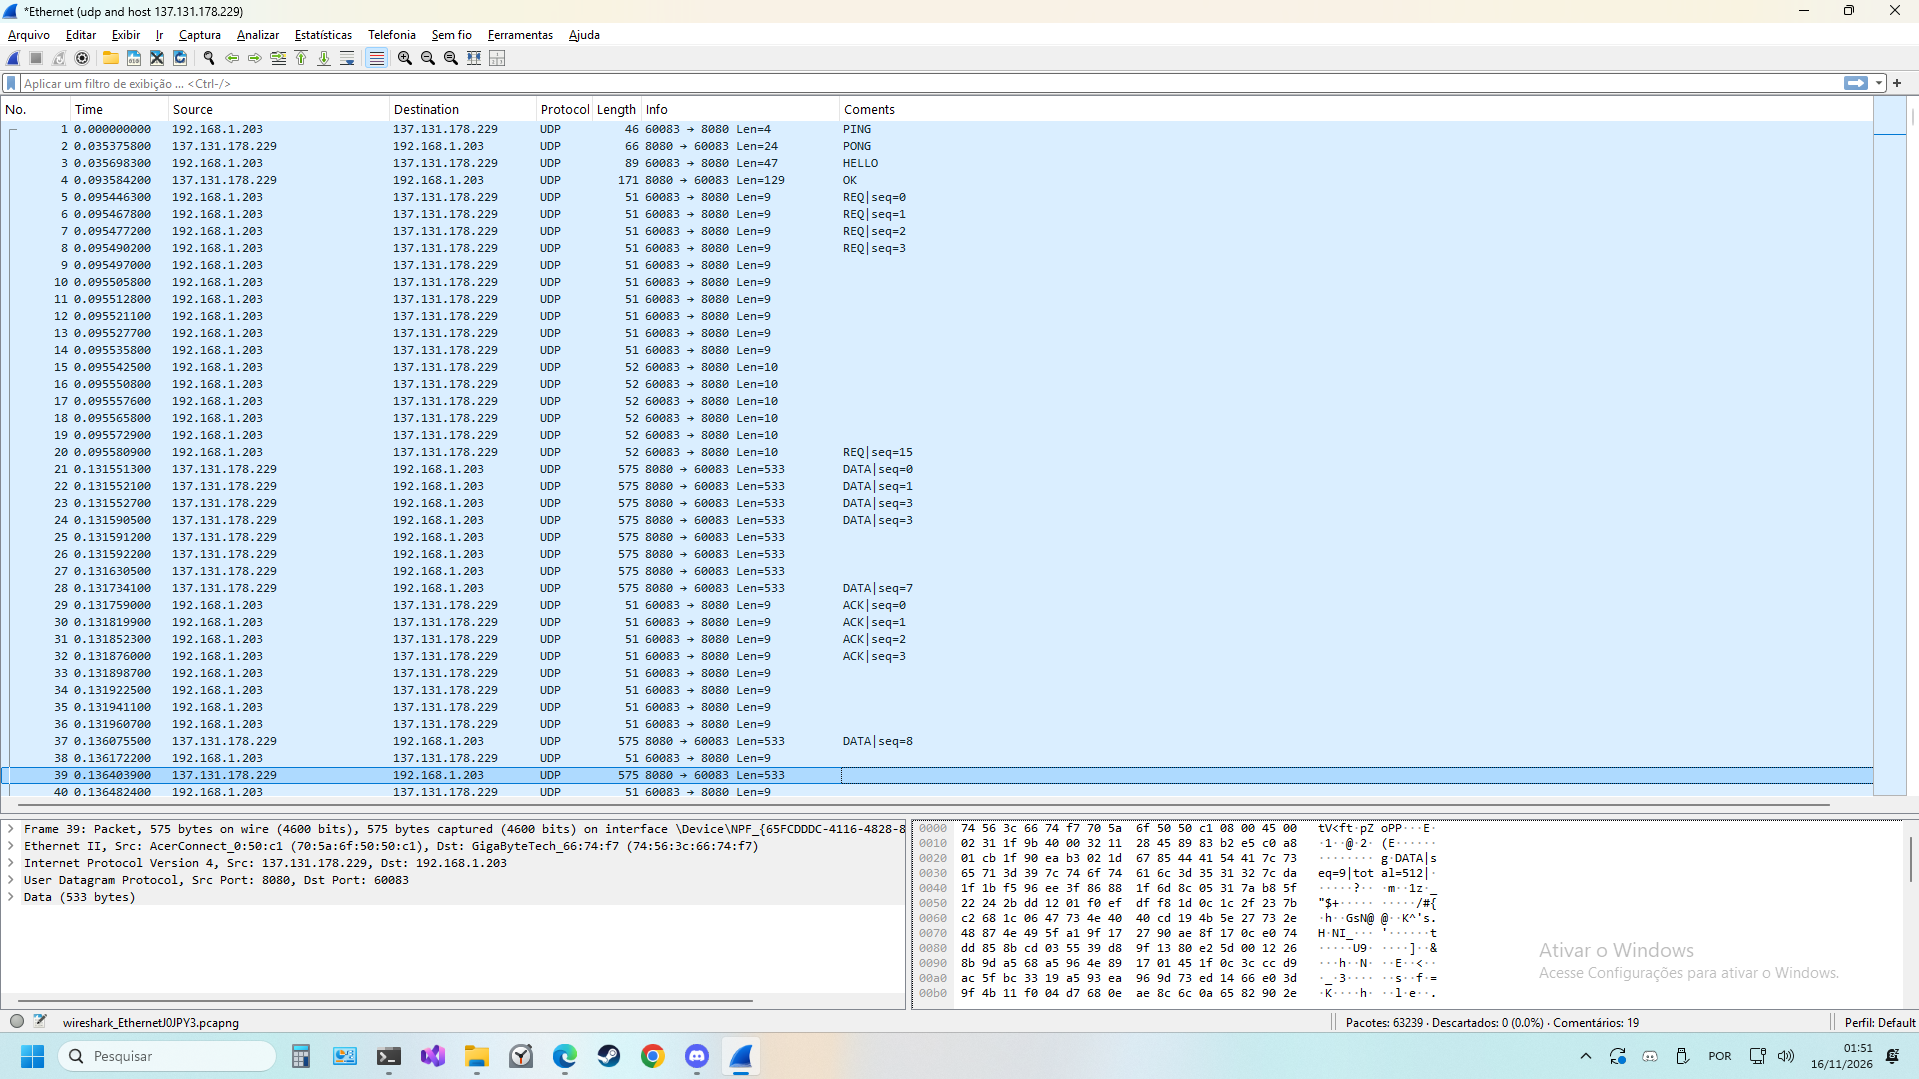
\includegraphics[width=0.9\linewidth]{imagens/wireshark_inicio.png}
\caption{Inicio da transferência no wireshark.}
\label{fig:wire_inicio}
\end{figure}

\begin{figure}[H]
\centering
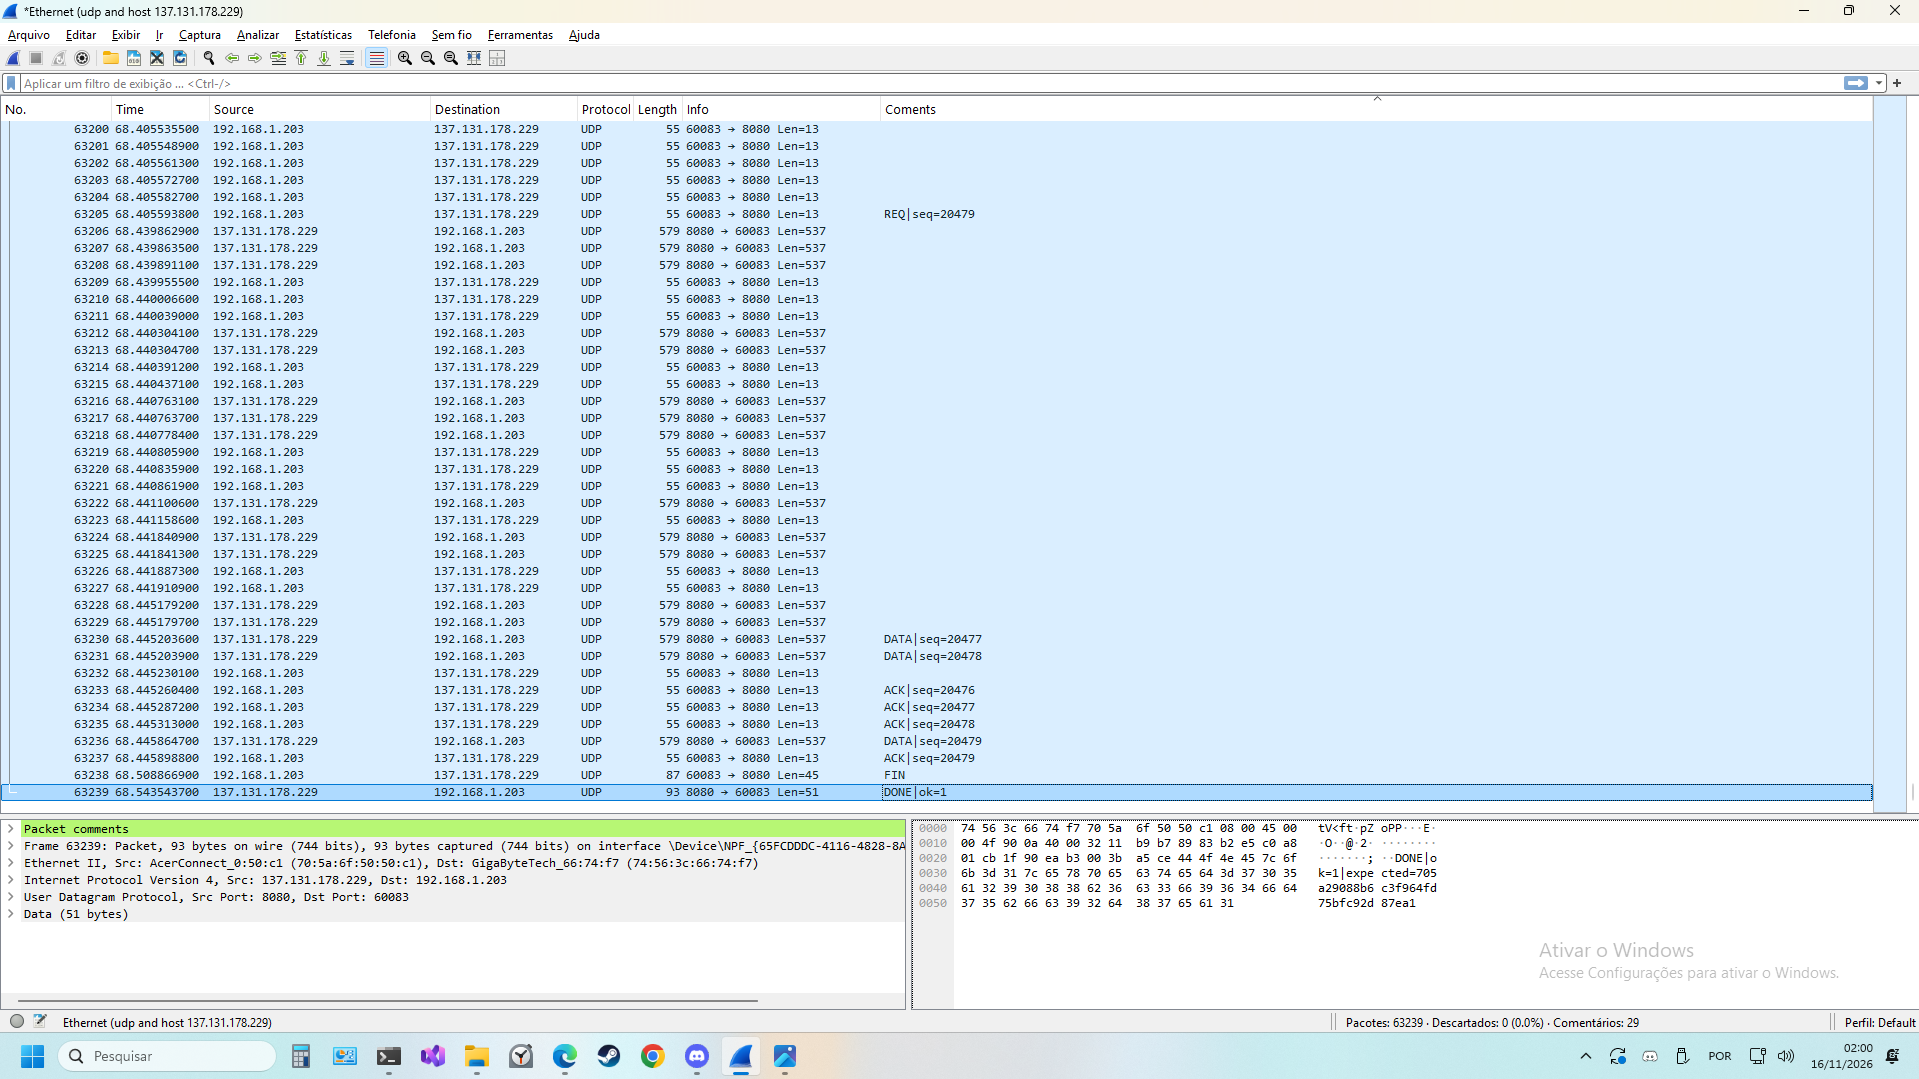
\includegraphics[width=0.9\linewidth]{imagens/wireshark_final.png}
\caption{Final da transferência. Nota-se o pacote DONE retornando ok=1 significando sucesso.}
\label{fig:wire_final}
\end{figure}

\begin{figure}[H]
\centering
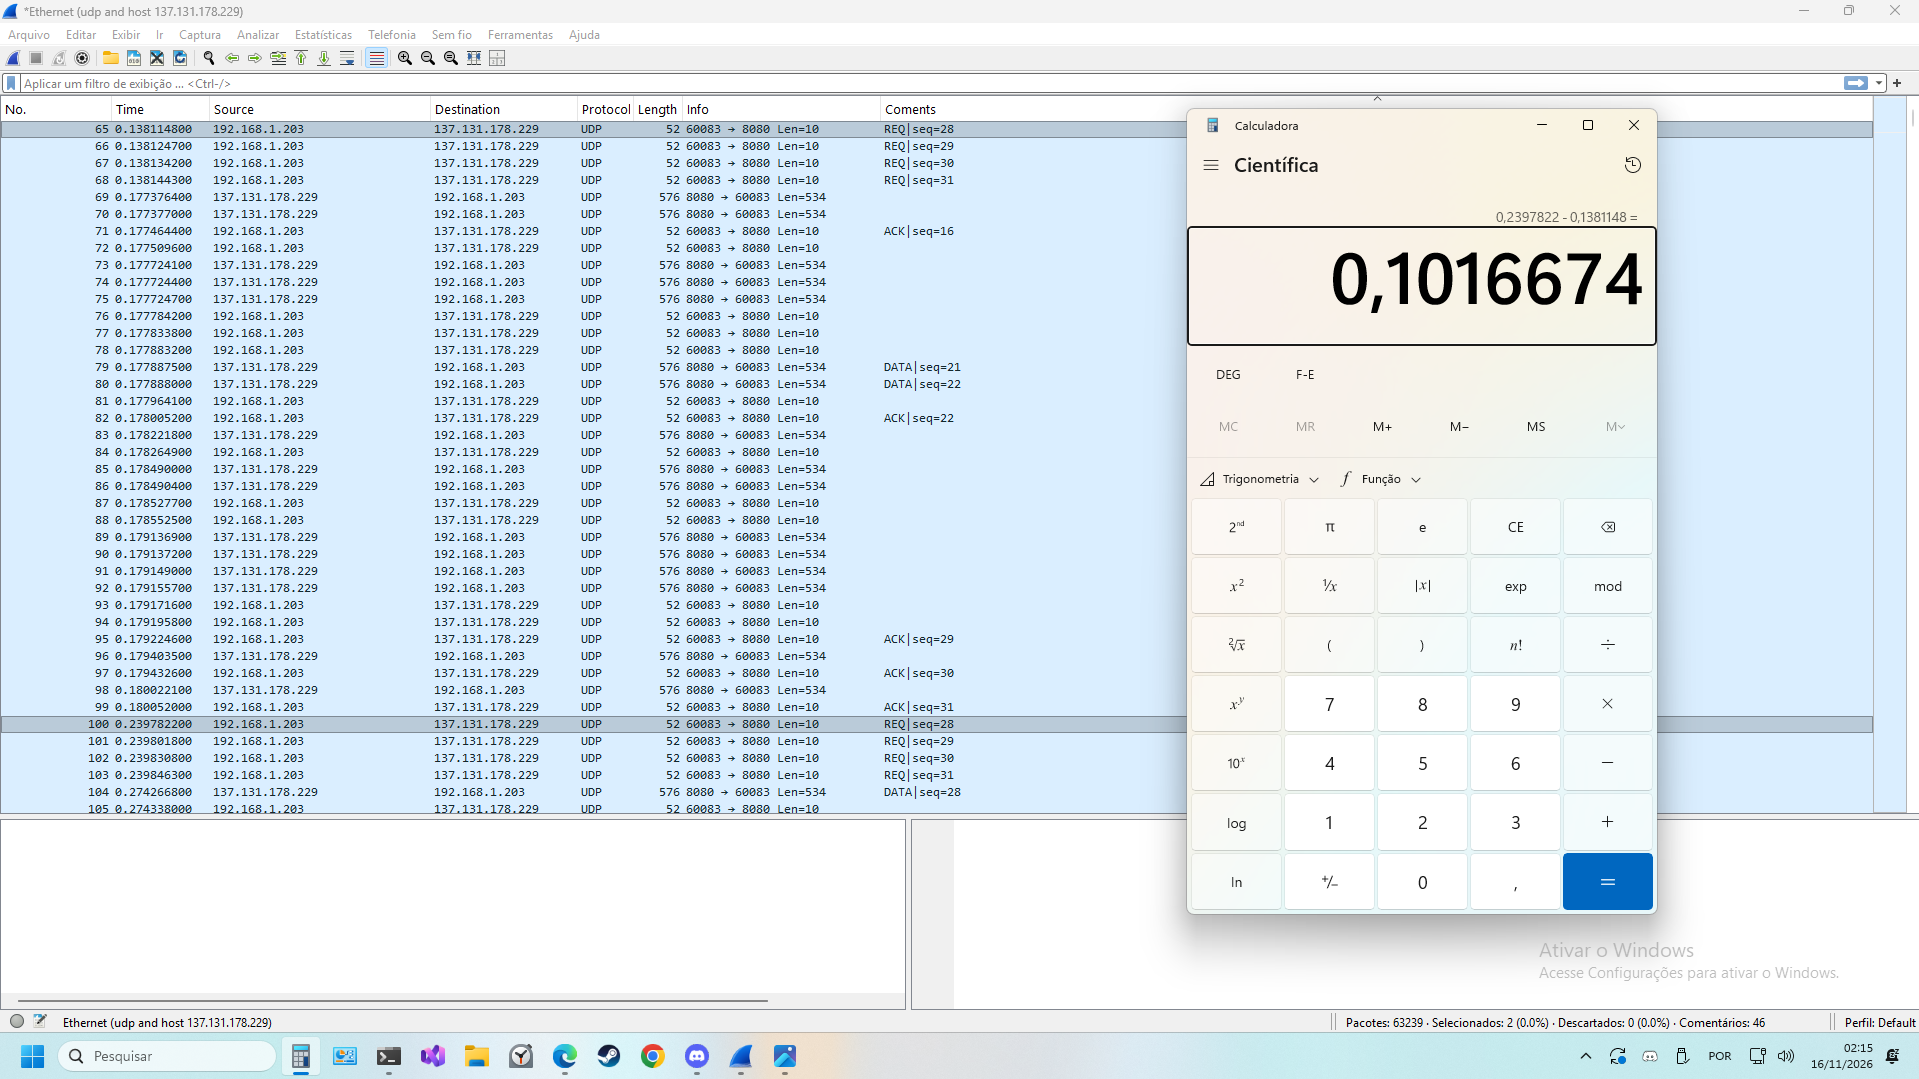
\includegraphics[width=0.9\linewidth]{imagens/wireshark_retransmissao.png}
	\caption{Situação de retransmissão. Em destaque, está a primeira solicitação e a segunda. Entre elas, ouve um timeout de \SI{101}{\milli\second}.}
\label{fig:wire_retra1}
\end{figure}

\begin{figure}[H]
\centering
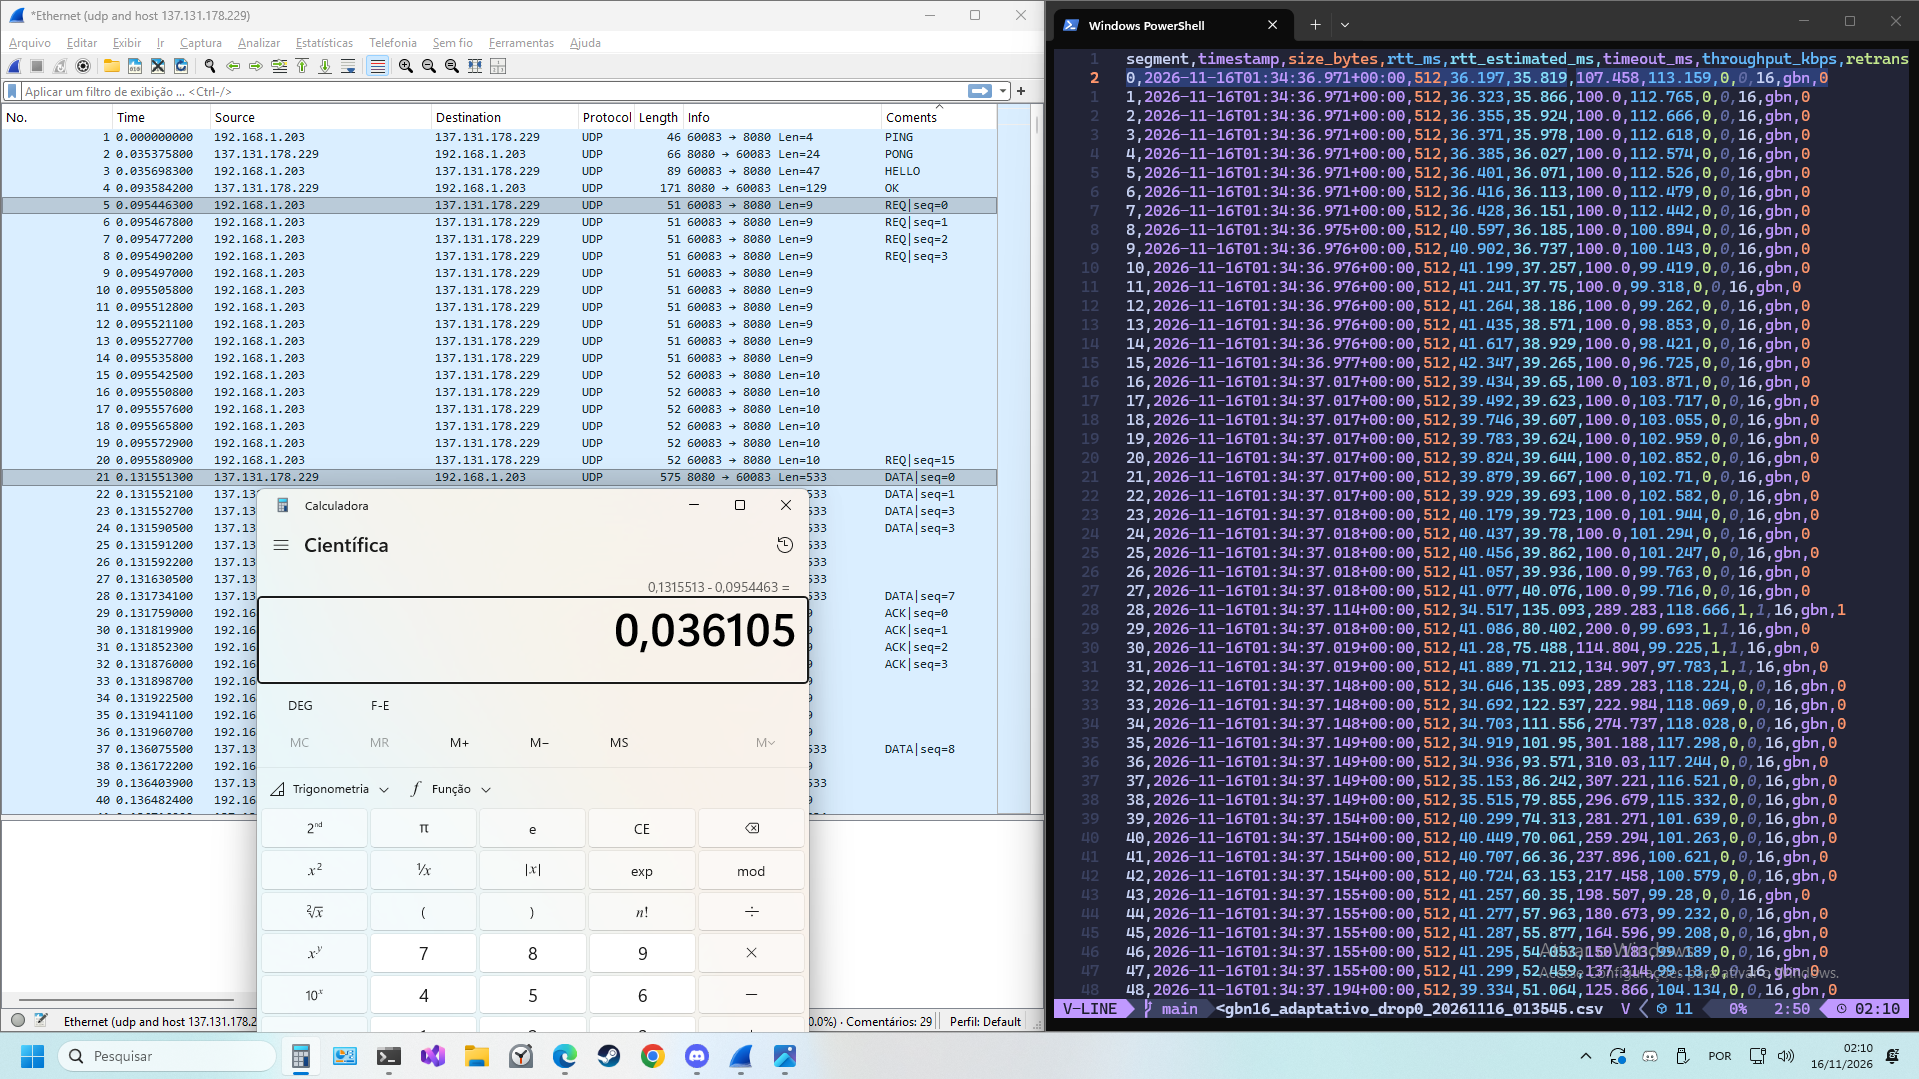
\includegraphics[width=0.9\linewidth]{imagens/wireshark_csv.png}
\caption{Uma requisição no Wireshark e no CSV mostrado lado a lado. Estão em destaque o pacote REQ e DATA do seq=0, e também a linha do CSV respectiva. O cálculo do
	RTT usando o wireshark resultou em \SI{36.1}{\milli\second} e o CSV registrou \SI{36.2}{\milli\second}. A diferença se dá ao fato de que o
	wireshark captura o pacote antes do programa em si ter acesso, fazendo-o ter uma leve vantagem em relação ao cliente.}
\label{fig:wire_csv}
\end{figure}

\section{Visão integrada}
\label{sec:integrada}

%%%%%%%%%%%%%%%%%%%%%%%%%%%%%%%%%%%%%%%%%%%%%%%%%%%%%%%%%%%%%%%%%%%%%%%%%%%%%%%%
% 5. Visão integrada — comparação final de todos os protocolos
%
% Tabela única consolidando os resultados das três entregas, com o melhor cenário de cada protocolo:
%
% Protocolo	Janela	Timeout	Throughput médio	Retransmissões	Tempo total (large)
% SAW	1	fixo	—	—	—
% GBN	16	fixo	—	—	—
% GBN	16	adaptativo	—	—	—
% SR	16	fixo	—	—	—
% SR	16	adaptativo	—	—	—
% Gráfico de barras comparando throughput médio de todos os protocolos — um único gráfico que conta a história do projeto inteiro.
%%%%%%%%%%%%%%%%%%%%%%%%%%%%%%%%%%%%%%%%%%%%%%%%%%%%%%%%%%%%%%%%%%%%%%%%%%%%%%%%

Esta tabela consolida todos os protocolos implementados e mostra a evolução do projeto.

\begin{table}[H]
\begin{center}
\begin{tabular}{@{}lrrrr@{}}
\toprule
	\textbf{Protocolo} & \textbf{Timeout} & \textbf{Throughput médio} & \textbf{Retransmissões} & \textbf{Tempo total (large)} \\
\midrule
	SAW    & fixo       & \SI{110.47}{\kilo\bit\per\second}  & 6  & \SI{759.34}{\second} \\
	GBN-16 & fixo       & \SI{1008.06}{\kilo\bit\per\second} & 0  & \SI{83.22}{\second} \\
	GBN-16 & adaptativo & \SI{1351.72}{\kilo\bit\per\second} & 0  & \SI{62.06}{\second} \\
	SR-16  & fixo       & \SI{1693.72}{\kilo\bit\per\second} & 8  & \SI{49.53}{\second} \\
	SR-16  & adaptativo & \SI{2089.87}{\kilo\bit\per\second} & 0  & \SI{40.07}{\second} \\

\bottomrule
\end{tabular}
\end{center}
	\caption{Dados de todos os protocolos desenvolvidos}
	\label{tab:dados_todos}
\end{table}

\begin{figure}[H]
\centering
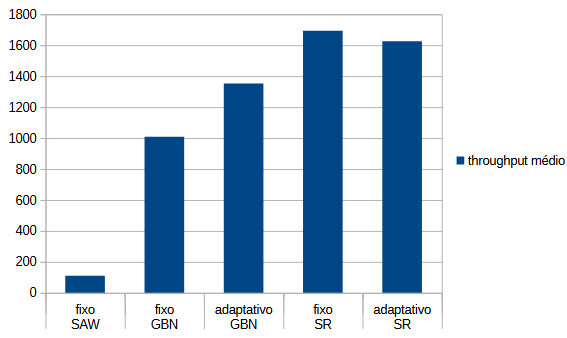
\includegraphics[width=0.8\linewidth]{imagens/grafico_barra_total.png}
\caption{Gráfico de barras do throughput médio observado para cada protocolo}
\label{fig:graf_barra_throughput}
\end{figure}

Ao analisá-la, é possível notar valores inesperados, por exemplo, os valores do throughput médio do GBN-16,
está bem menor que o SR-16 mesmo considerando que o primeiro não houve retransmissões. Isso se deve ao fato
de que estes protocolos, mesmo com todos os avanços, ainda são extremamente suscetíveis ao RTT. Quando os
testes foram realizados para o GBN-16, o RTT médio flutuou entre \SI{48}{\milli\second} e \SI{62}{\milli\second}, enquanto o
SR-16 teve um RTT médio de \SI{39}{\milli\second}. Isso não são falhas dos algorítimos e sim reflexo da
flutuabilidade da rede nos computadores onde foram realizados os testes.

Uma ressalva importante sobre as medições de timeout adaptativo desta tabela: as
execuções sem perda foram refeitas depois da correção do backoff — a versão
anterior dobrava também o estimador EWMA a cada timeout, contaminando-o
permanentemente, e chegou a medir SR-16 adaptativo abaixo do fixo
(\SI{1625.88}{\kilo\bit\per\second}) mesmo sem perdas. Com o backoff corrigido
(RFC 6298: dobra apenas o RTO, o estimador fica intacto), o SR-16 adaptativo
fez \SI{2089.87}{\kilo\bit\per\second} com zero retransmissões — a diferença
para o fixo, \SI{1693.72}{\kilo\bit\per\second}, reflete sobretudo o RTT médio
da sessão (31,2~ms contra 39~ms), e não a regra do timeout, que nunca estourou
em nenhuma das duas. Sob perda, a vantagem do adaptativo é real e grande
(Seção~\ref{sec:fixo_adapt}): \SI{57}{\percent} a \SI{5}{\percent} de perda e
\SI{116}{\percent} a \SI{10}{\percent}. Sem perdas, o fixo é suficiente; com
perdas, ele desperdiça \SI{500}{\milli\second} por evento, contra ~\SI{100}{\milli\second}
do adaptativo.


\section{Conclusão}
Ao longo das três etapas deste projeto, foi possível compreender de forma prática os desafios associados ao desenvolvimento de protocolos de transferência confiável de dados sobre redes IP/UDP. A evolução do modelo básico Stop-and-Wait (SAW) até os protocolos de janela deslizante (Go-Back-N e Selective Repeat) com estimativa dinâmica de RTT evidenciou a importância de mecanismos inteligentes de controle de fluxo e retransmissão.

No ambiente de testes utilizando o servidor remoto, o Selective Repeat (SR) com janela de tamanho 16 e o uso de RTT adaptativo apresentou o melhor desempenho geral, especialmente em cenários com perdas de pacotes. Enquanto o SAW apresentou limitações severas de largura de banda devido à ociosidade do canal, e o GBN sofreu quedas expressivas de vazão por descartar pacotes corretos após uma perda isolada, o SR demonstrou maior resiliência e eficiência na utilização do canal.

A introdução do algoritmo de RTT adaptativo baseado em EWMA (com $\alpha = 0.125$ e $\beta = 0.25$) agregou valor substancial ao projeto, eliminando a necessidade de adivinhar um valor de timeout estático que frequentemente resultava em retransmissões prematuras desnecessárias ou esperas excessivas em caso de oscilações na rede. Com a mesma sequência de perdas (mesma seed), o SR-16 adaptativo atingiu \SI{1525}{\kilo\bit\per\second} contra \SI{705}{\kilo\bit\per\second} do fixo a \SI{10}{\percent} de perda — mais que o dobro — e \SI{1789}{\kilo\bit\per\second} contra \SI{1139}{\kilo\bit\per\second} a \SI{5}{\percent}; sem perdas os dois empatam, pois o timer simplesmente não estoura. A implementação exigiu ainda o refinamento do backoff para a forma correta da RFC 6298 (dobrar apenas o RTO, sem contaminar o estimador EWMA), sem o qual os picos de backoff se espalhavam pela sessão inteira. A complexidade adicional foi amplamente compensada pela adaptação dinâmica do temporizador às condições reais de tráfego.

Caso o projeto fosse reiniciado, o grupo priorizaria a estruturação modular da camada de transporte desde a primeira entrega, facilitando a reutilização de componentes de controle de socket e logging de métricas, a implementação de uma interface visual interativa no terminal (como uma barra de progresso dinâmica em tempo real para acompanhar a transferência dos pacotes), e o planejamento de testes automatizados mais abrangentes para validar o comportamento dos temporizadores sob diferentes perfis de ruído e atraso na rede.

%%%%%%%%%%%%%%%%%%%%%%%%%%%%%%%%%%%%%%%%%%%%%%%%%%%%%%%%%%%%%%%%%%%%%%%%%%%%%%%%
% 6. Conclusão
%
% Qual protocolo teve melhor desempenho no ambiente do projeto (rede real, RTT ~22ms)?
% O RTT adaptativo valeu a complexidade adicional de implementação? Justifique com dados.
% O que o grupo implementaria diferente se fosse recomeçar?
%%%%%%%%%%%%%%%%%%%%%%%%%%%%%%%%%%%%%%%%%%%%%%%%%%%%%%%%%%%%%%%%%%%%%%%%%%%%%%%%

\section{Referências}

\begin{referencias}
\item James F. Kurose \& Keith W. Ross, \emph{Redes de Computadores e a Internet - Uma nova Abordagem}, 8a Edição, Pearson Education / Makron Books.

\item Andrew S. Tanenbaum, \emph{Redes de Computadores}, Pearson Universidades, 5a Edição, 2011
\end{referencias}

\end{document}
